\subsection{Introducci\'on a los aut\'omatas celulares} 
    \label{sec:AutomatasCelulares}
    % Parrafo 1
    Primero es necesario conocer la teor\'ia de aut\'omatas y como se relaciona con los aut\'omatas celulares,
        por ello daremos un breve repaso de la teor\'ia de aut\'omatas.
    \vskip 0.5cm
    \subsubsection{Teor\'ia de Aut\'omatas}
    \label{sec:TeoriaAutomatas}
    % Parrafo 1
    La teor\'ia de aut\'omatas es el estudio de dispositivos de c\'alculo abtractos, es decir de las m\'aquinas.\cite{Hopcroft1979}
        Estos aut\'omatas son modelos matem\'aticos fundamentales en el \'area de estudio de las ciencias de la computaci\'on, 
        son usados para entender los procesos de c\'alculo y toma de decisiones. En la teor\'ia de aut\'omatas se estudian
        los aut\'omatas finitos, los aut\'omatas con pila, las m\'aquinas de Turing, los aut\'omatas celulares, etc.
        Los aut\'omatas regulares pueden ser jerarquizados en una jerarqu\'ia de Chomsky\cite{Aranda2006}, que es una jerarqu\'ia de lenguajes formales.
        La cual ser\'ia la siguiente:
        \begin{itemize}
            \item \textbf{Tipo 3 - Gram\'aticas regulares:} Estos generan los lenguajes regulares.
                Estas se restrinjen a producciones de la forma $A \rightarrow a\gamma$ y $A \rightarrow aB$. Son 
                asociados a los aut\'omatas finitos.
            \item \textbf{Tipo 2 - Gram\'aticas libres de contexto:} Estos generan los lenguajes independientes del contexto.
                Estas se restrinjen a producciones de la forma $A \rightarrow \gamma$. Son asociados a los aut\'omatas con pila.
            \item \textbf{Tipo 1 - Gram\'aticas sensibles al contexto:} Estos generan los lenguajes sensibles al contexto.
                Estas se restrinjen a producciones de la forma ${\alpha}A{\beta} \rightarrow {\alpha}{\gamma}{\beta}$. 
                Son asociados a las m\'aquinas de Turing linealmente acotadas (significa que la cinta de la m\'aquina de Turing
                tiene un l\'imite derterminada por un cierto n\'umero entero de veces sobre la longitud de entrada).
            \item \textbf{Tipo 0 - Gram\'aticas irrestrictas:} Estos generan los lenguajes recursivamente enumerables.
                Estas se restrinjen a producciones de la forma ${\alpha}A{\beta} \rightarrow {\delta}$. Son asociados a las m\'aquinas de Turing.
        \end{itemize}
    % Parrafo 2
    \vskip 0.5cm
    En cambio los aut\'omatas celulares, aunque diferentes en estructura y aplicaci\'on a las gram\'aticas formales, 
        tambi\'en son modelos matem\'aticos fundamentales en el \'area de estudio de las ciencias de la computaci\'on
        y forman parte de la teor\'ia de aut\'omatas. Mientras que los aut\'omatas convencionales se centran en el procesamiento 
        secuencial de cadenas de s\'imbolos y operan bas\'andose en estados y transiciones claramente definidos, los aut\'omatas 
        celulares utilizan una red de c\'elulas cuyos estados evolucionan en paralelo, siguiendo reglas locales. Esta diferencia 
        fundamental en su enfoque los hace especialmente adecuados para modelar y explorar fen\'omenos que involucran procesos din\'amicos 
        y patrones espaciales. A pesar de estas diferencias, los aut\'omatas celulares se alinean con los principios fundamentales de la 
        teor\'ia de aut\'omatas en cuanto a la representaci\'on y manipulaci\'on de informaci\'on, ofreciendo una perspectiva m\'as amplia y diversa 
        sobre lo que constituye un \textit{`aut\'omata'} en el contexto de la computaci\'on y el procesamiento de informaci\'on. Su inclusi\'on en la teor\'ia 
        de aut\'omatas subraya la amplitud y la profundidad de este campo, demostrando que la teor\'ia de aut\'omatas no solo se limita a las m\'aquinas 
        y lenguajes formales tradicionales, sino que tambi\'en abarca modelos computacionales m\'as generales y vers\'atiles.
    % Parrafo 2
    \vskip 0.5cm
    Una vez que hemos explicado la teor\'ia de automatas podemos pasar a explicar en mas detalle los aut\'omatas celulares.
    \vskip 0.5cm
    \subsubsection{Aut\'omatas celulares de una dimensi\'on}
\label{sec:AutomatasCel1D}
%Parrafo 1
    Los aut\'omatas celulares de una dimensi\'on consisten de una linea de celdas o estados, cada una con 2 estados posibles, 
        0 o 1, vivo o muerto, etc. Estas celdas se actualizan en cada generaci\'on, de acuerdo a una regla de evoluci\'on, 
        la cual determina el estado de una celda en la siguiente generaci\'on, bas\'andose en el estado de la celda y sus 
        vecinos en la generaci\'on actual. La regla de evoluci\'on se aplica a todas las celdas de la misma manera, y en 
        paralelo, es decir, todas las celdas se actualizan al mismo tiempo. Para ejemplificar esto, se puede ver la Figura
        \ref{fig:automataCelular1D}. En donde tenemos la regla de evoluci\'on 30, de las \textit{Reglas de Wolfram}\cite{Wolfram1959}, o
        \textit{Automatas Celulares Elementales} (Elemental Cellular Automata, ECA), en la cual se puede ver que la celda de la generaci\'on $t+1$ depende
        de la celda de la generaci\'on $t$ y sus vecinos.
        \begin{figure}[h!]
            \centering
            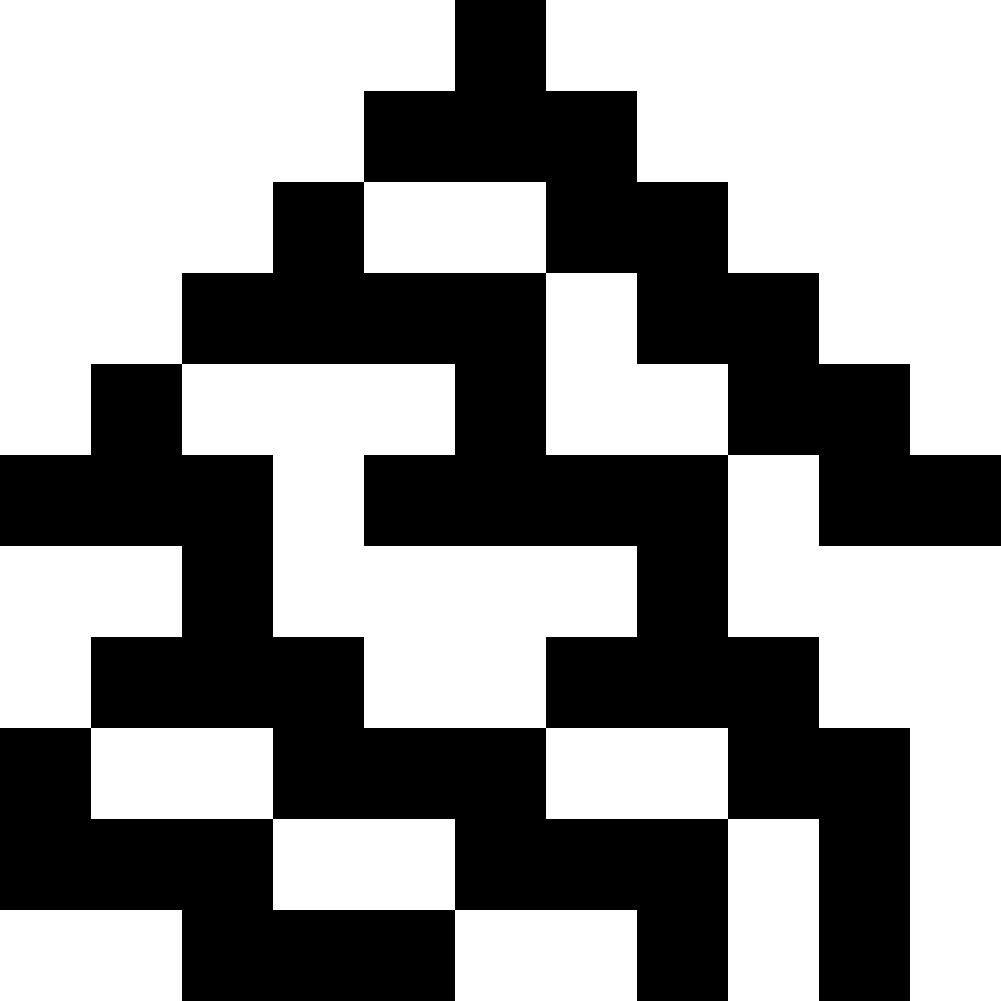
\includegraphics[width=0.5\textwidth]{./images/marco_teorico/automatas_celulares/Regla30.png}
            \caption{Regla de evoluci\'on 30 de las \textit{Reglas de Wolfram} 10 generaciones o (t)}
            \label{fig:automataCelular1D}
        \end{figure}
%Parrafo 2
    \vskip 0.5cm
    Como podemos ver en estos aut\'omatas celulares de una dimensi\'on los que podemos considerar los elementos m\'as importantes son:
        \begin{itemize}
            \item \textbf{Vecindad:} Es el conjunto de celdas que se toman en cuenta para la actualizaci\'on de una celda.
            \item \textbf{Estado:} Es el valor que puede tomar una celda, en este caso solo puede ser 0 o 1.
            \item \textbf{Regla de evoluci\'on:} Es la regla que determina el estado de una celda en la siguiente generaci\'on.
        \end{itemize}
    \vskip 0.5cm
    En este caso la vecindad la forman la celda y sus dos vecinos, pero puede ser de cualquier tama\~no, siempre y cuando
        sea sim\'etrica, es decir, que la celda se encuentre en el centro de la vecindad. El estado de la celda puede ser
        cualquier valor, pero en este caso solo puede ser 0 o 1. La regla de evoluci\'on es la que determina el estado de
        la celda en la siguiente generaci\'on, en este caso la regla de evoluci\'on 30, que se puede ver en la Figura
        \ref{fig:automataCelular1D}, es la siguiente:
        \begin{table}[h!]
            \centering
            \begin{tabular}{|c|c|c|c|c|c|c|c|}
                \hline
                \textbf{111} & \textbf{110} & \textbf{101} & \textbf{100} & \textbf{011} & \textbf{010} & \textbf{001} & \textbf{000} \\
                \hline
                0 & 0 & 0 & 1 & 1 & 1 & 1 & 0 \\
                \hline
            \end{tabular}
            \caption{Regla de evoluci\'on 30}
            \label{tab:reglaEvolucion30}
        \end{table}
    \vskip 0.5cm
    Como podemos ver en el Cuadro \ref{tab:reglaEvolucion30} la regla de evoluci\'on 30 es una regla de evoluci\'on local, 
        es decir, que solo depende de la celda y sus vecinos, y no de toda la l\'inea de celdas. En este caso la regla de evoluci\'on
        30 es una regla de evoluci\'on determinista, es decir, que para una celda y sus vecinos siempre se obtiene el mismo resultado.
        Pero tambi\'en existen las reglas de evoluci\'on no deterministas, en las cuales para una celda y sus vecinos se puede obtener
        m\'as de un resultado. En este caso la regla de evoluci\'on 30 es una regla de evoluci\'on unidimensional, es decir, que la
        celda solo depende de sus vecinos de la izquierda y de la derecha, pero tambi\'en existen las reglas de evoluci\'on
        bidimensionales, n-dimensionales, etc.
    \vskip 0.5cm
    \subsubsection{Condiciones frontera}
        Por definici\'on los aut\'omatas celulares son infinitos, pero en la pr\'actica no se pueden tener aut\'omatas celulares
            infinitos, por lo que se tienen que definir condiciones frontera, las cuales son las condiciones que se tienen en los
            extremos del aut\'omata celular. Existen diferentes tipos de condiciones frontera, las cuales son:
            \vskip 0.5cm
        \begin{wrapfigure}{r}{0.25\textwidth}
            \centering
            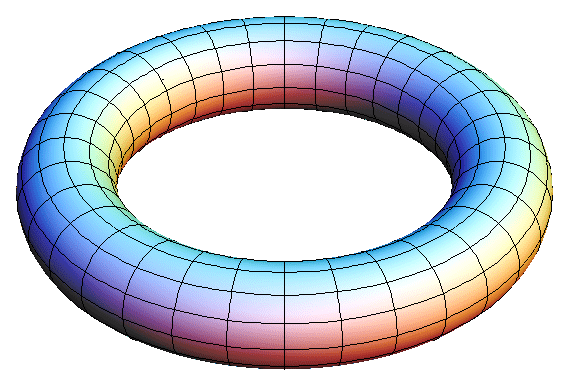
\includegraphics[width=0.25\textwidth]{./images/marco_teorico/automatas_celulares/torus.png}
            \caption{Representaci\'on de un toroide \cite{Sharma2022}}
            \label{fig:toroide}
        \end{wrapfigure}
        \begin{itemize}
            \item \textbf{Abierta} En este caso las celdas de los extremos no tienen vecinos, por lo que no se pueden actualizar.
            \item \textbf{Peri\'odica} En este caso las celdas de los extremos tienen como vecinos a las celdas del otro extremo.
            \item \textbf{Reflejante} En este caso las celdas de los extremos tienen como vecinos a las celdas del otro extremo, pero
                invertidas.
            \item \textbf{Frontera} En este caso las celdas de los extremos tienen como vecinos a celdas con un valor fijo.
        \end{itemize}
    \vskip 0.5cm
    En nuestro caso, utilizaremos la condici\'on frontera peri\'odica; esta tiene forma de un toroide, como se puede ver en la Figura
        \ref{fig:toroide}.
        \vskip 0.5cm
        
        Tambi\'en podemos observar que en la Figura \ref{fig:toroide} se puede ver que las celdas de los extremos tienen como
            vecinos a las celdas del otro extremo, por lo que se puede decir que es una condici\'on frontera peri\'odica.
        \vskip 0.5cm
    \subsubsection{Vecindario}
    \label{sec:Vecindario}
    Un vecindario es un conjunto de celdas que se toman en cuenta para la actualizaci\'on de una celda. Como vimos con anterioridad
        en los aut\'omatas celulares de una dimensi\'on, el vecindario de una celda es la celda y sus dos vecinos, pero en los aut\'omatas
        celulares de dos dimensiones el vecindario de una celda puede ser de cualquier tama\~no, siempre y cuando sea sim\'etrico, es decir,
        que la celda se encuentre en el centro del vecindario. En la Figura \ref{fig:mooreN} se puede ver un ejemplo de un vecindario
        de una celda. E incluso en los aut\'omatas celulares de dos dimensiones se pueden tener vecindarios de diferentes formas, como se
        es com\'un verlos en forma cuadrada y en forma hexagonal, as\'i como se muestra en las Figuras \ref{fig:mooreN} - \ref{fig:hexN}.
    \vskip 0.5cm
    A su vez los vecindarios m\'as usados son los siguientes: 
    \begin{itemize}
        \item 
            \begin{minipage}
                {0.5\textwidth}
                \textbf{Vecindario de Moore} En este caso el vecindario de una celda es la celda y sus ocho vecinos.
            \end{minipage}
            \begin{minipage}{0.5\textwidth}
                \centering
                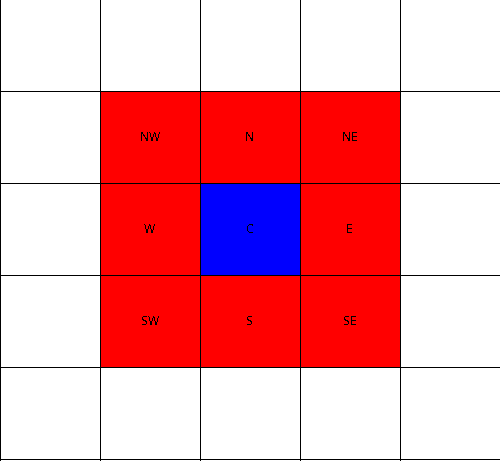
\includegraphics[width=0.5\textwidth]{./images/marco_teorico/automatas_celulares/mooreN.png}
                \captionof{figure}{Vecindario de Moore}
                \label{fig:mooreN}
            \end{minipage}
        \item
            \begin{minipage}
                {0.5\textwidth}
                \textbf{Vecindario de von Neumann} En este caso el vecindario de una celda es la celda y sus cuatro vecinos.
            \end{minipage}
            \begin{minipage}
                {0.5\textwidth}
                \centering
                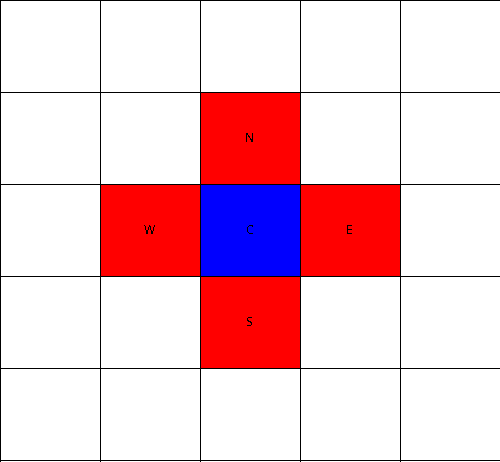
\includegraphics[width=0.5\textwidth]{./images/marco_teorico/automatas_celulares/vonN.png}
                \captionof{figure}{Vecindario de von Neumann}
                \label{fig:vonN}
            \end{minipage}
        \item
            \begin{minipage}
                {0.5\textwidth}
                \textbf{Vecindario de Moore extendido} En este caso el vecindario de una celda es la celda y sus veinticuatro vecinos.
            \end{minipage}
            \begin{minipage}
                {0.5\textwidth}
                \centering
                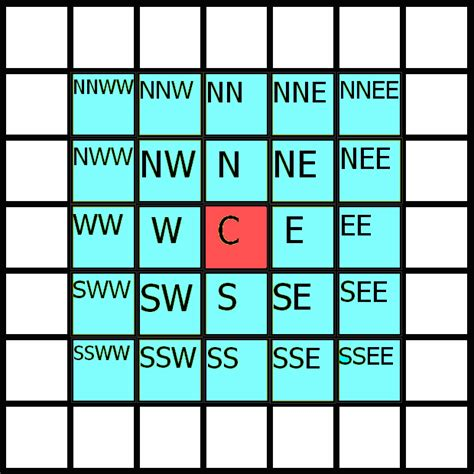
\includegraphics[width=0.5\textwidth]{./images/marco_teorico/automatas_celulares/mooreNeX.jpg}
                \captionof{figure}{Vecindario de Moore extendido}
                \label{fig:mooreNeX}
            \end{minipage}
        \item 
            \begin{minipage}
                {0.5\textwidth}
                \textbf{Vecindario de von Neumann extendido} En este caso el vecindario de una celda es la celda y sus doce vecinos.
            \end{minipage}
            \begin{minipage}
                {0.5\textwidth}
                \centering
                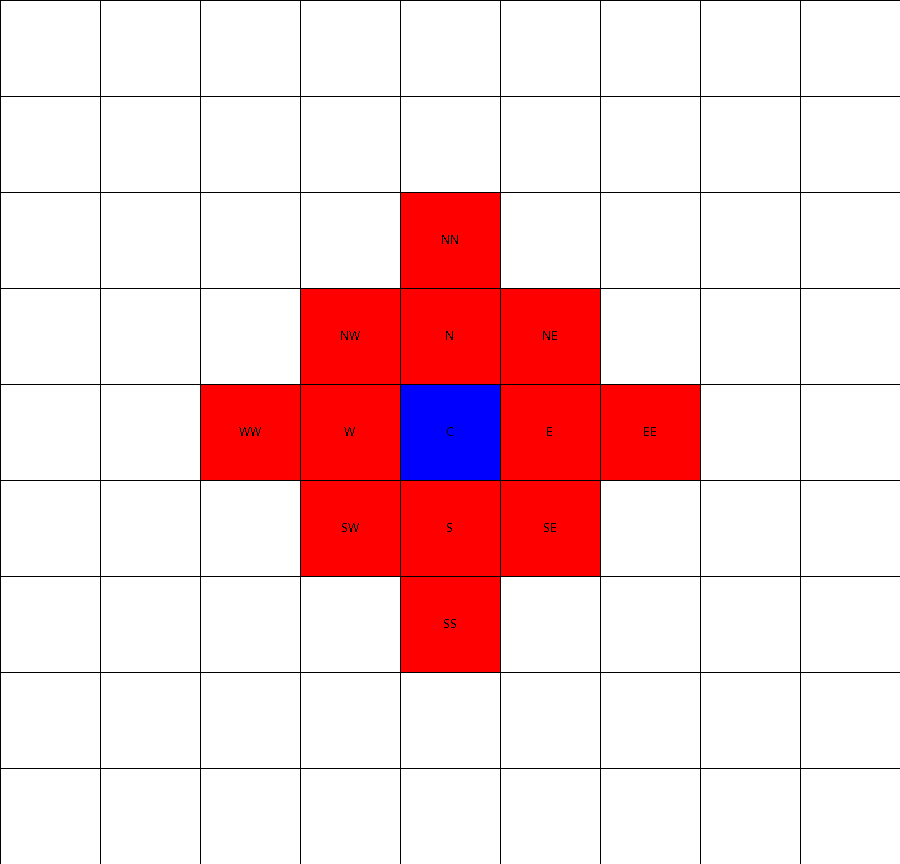
\includegraphics[width=0.5\textwidth]{./images/marco_teorico/automatas_celulares/vonNeX.png}
                \captionof{figure}{Vecindario de von Neumann extendido}
                \label{fig:vonNeX}
            \end{minipage}
        \item
            \begin{minipage}
                {0.5\textwidth}
                \textbf{Vecindario de hexagonal} En este caso el vecindario de una celda es la celda y sus seis vecinos.
            \end{minipage}
            \begin{minipage}
                {0.5\textwidth}
                \centering
                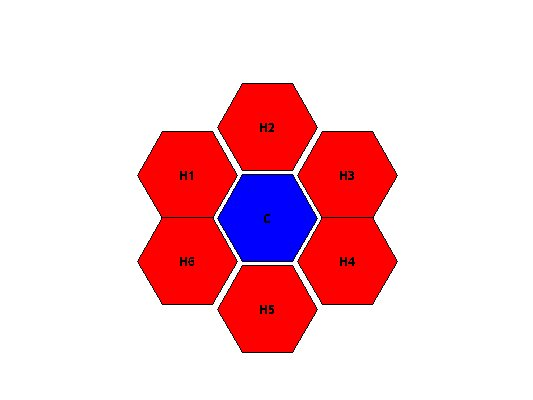
\includegraphics[width=0.5\textwidth]{./images/marco_teorico/automatas_celulares/hexN.jpg}
                \captionof{figure}{Vecindario de hexagonal}
                \label{fig:hexN}
            \end{minipage}
    \end{itemize}
    \vskip 0.5cm
    Una vez que hemos explicado eso podemos pasar a definir formalmente los aut\'omatas celulares.
    \vskip 0.5cm
    \subsubsection{Definici\'on formal}
    \label{sec:AutomatasCelDefFormal}
    Primero denotemos $\mathbb{Z}$ como el conjunto de los n\'umeros enteros, es decir, $\mathbb{Z} = (-\infty,-1 ,0,1, \infty)$.
        y la longitud de cualquier tupla $x$ como $|x|$. Para todas las tuplas $x$ y $y$ de la misma longitud, denotemos $x \oplus y$
        como la tupla que resulta de la suma componente a componente de $x$ y $y$, es decir, $(x \oplus y)_i = x_i + y_i$ para todo 
        $i \in \mathbb{Z}$.
    \vskip 0.5cm
    Entonces tenemos que un aut\'omata celular es una tupla $({\mathbb{Z}^{n}},S,N,f)$ tal que la $n$ dimensi\'on es al menos $1$ donde 
        $n \in \mathbb{Z}^{+}$, $S$ es un conjunto finito no vac\'io de estados, $N$ es un conjunto finito no vac\'io de vecindades 
        perteneciente a ${\mathbb{Z}^{n}}$ y $f$ es una funci\'on de transici\'on local, es decir, $f: S^N \rightarrow S$ donde
        $S^N$ representa al conjunto de todas las posibles configuraciones de vecindad en $N$.
    \vskip 0.5cm
    La configuraci\'on inicial de un aut\'omata celular es una funci\'on $c: {\mathbb{Z}^{n}} \rightarrow S$ que asigna un estado a cada celda.
        La evoluci\'on de un aut\'omata celular es una funci\'on $F: S^{{\mathbb{Z}^{n}}} \rightarrow S^{{\mathbb{Z}^{n}}}$ que asigna una configuraci\'on a la siguiente
        configuraci\'on, es decir, $F(c) = c'$, donde $c'$ es la configuraci\'on resultante de aplicar la funci\'on de transici\'on local a cada
        celda de la configuraci\'on $c$, es decir, $c'(x) = f(c|_{x+N})$ para todo $x \in {\mathbb{Z}^{n}}$, donde $c|_{x+N}$ es la restricci\'on de $c$ a la vecindad $x+N$.
        Esto tambi\'en aplica $n$ dimensionalmente, es decir, que se podr\'ia decir que $c'(x,y) = f(c|_{(x,y)+N})$ para todo $(x,y) \in {\mathbb{Z}^{2}}$.
        Otra notaci\'on que podemos usar, y de hecho es la que utilizaremos es $C(x,y:t)$ donde $C$ es el centro de la vecindad, $x$,$y$ son las coordenadas de la celda y $t$ es el tiempo,
        o generaciones.
    \vskip 0.5cm
    Cabe a\~nadir que puede haber reestricciones adicionales en el conjunto de vecindades $N$ y en la funci\'on de transici\'on local $f$.
        Por ejemplo, en el caso de los aut\'omatas celulares de una dimensi\'on, el conjunto de vecindades $N$ es un conjunto de tuplas de longitud 3,
        donde la primera componente es la celda, la segunda componente es la celda de la izquierda y la tercera componente es la celda de la derecha.
        Y la funci\'on de transici\'on local $f$ es una funci\'on de 8 variables booleanas, es decir, $f: \{0,1\}^3 \rightarrow \{0,1\}$.
    \vskip 0.5cm    
    Y en el caso de los aut\'omatas celulares de dos dimensiones, el conjunto de vecindades $N$ es un conjunto de tuplas de longitud variable, 
        dependiendo del tipo de vecindad, donde la primera componente es la celda y las dem\'as componentes son las celdas vecinas. Por ejemplo, 
        en el caso de la vecindad de Moore, el conjunto de vecindades $N$ es un conjunto de tuplas de longitud 9, donde la primera componente es la celda
        $(x,y)$ el cual ser\'ia el centro de la vecindad, la segunda componente es la celda $(x-1,y-1)$, la tercera componente es la celda $(x-1,y)$,
        la cuarta componente es la celda $(x-1,y+1)$, la quinta componente es la celda $(x,y-1)$, la sexta componente es la celda $(x,y+1)$, la s\'eptima
        componente es la celda $(x+1,y-1)$, la octava componente es la celda $(x+1,y)$ y la novena componente es la celda $(x+1,y+1)$. Aqu\'i 
        $(x,y)$ es la celda central de la vecindad. Y la funci\'on de transici\'on local $f$ es una funci\'on de 512 variables booleanas, es decir,
        $f: \{0,1\}^{9} \rightarrow \{0,1\}$.
    \vskip 0.5cm
    Esta definici\'on formal de aut\'omata celular fue tomada de \cite{Codd1968}. Una vez explicada la definici\'on formal de aut\'omata celular,
        podemos pasar a explicar a m\'as detalle los aut\'omatas celulares de 2 dimensiones, los cuales son los que se usan en este trabajo terminal.
    \vskip 0.5cm
    \subsubsection{Aut\'omatas celulares de 2 Dimensiones}
\label{sec:AutomatasCel2D}

    %Parrafo 1
    Los aut\'omatas celulares de 2 dimensiones son los que se usan en este trabajo terminal, por ello es necesario
        explicarlos con m\'as detalle. Primero recordando lo ya explicado en anteriores subsecciones, un aut\'omata
        celular de 2 dimensiones es una tupla $({\mathbb{Z}^{2}},S,N,f)$\ref{sec:AutomatasCelDefFormal} y este 
        necesita de 8 elementos para poder ser definido, los cuales son los siguientes:         
    \begin{enumerate}
        \item \textbf{Celdas}: Es la unidad b\'asica del aut\'omata celular. Cada celda ocupa una posici\'on en el espacio, 
            para ser representados suelen usarse cuadr\'iculas o redes, esta tiene un estado y una vecindad.
        \item \textbf{Estados}: Cada celda puede estar en uno de varios estados posibles. En los aut\'omatas celulares
            m\'as simples, cada celda puede estar en uno de dos estados posibles (0 o 1, vivo o muerto, etc), pero en los 
            aut\'omatas celulares m\'as complejos, cada celda puede estar en uno de varios estados posibles. En el caso 
            en particular del Physarum polycephalum, cada celda puede estar en uno de nueve estados posibles 
            $\mathbb{P} = \{x \in \mathbb{Z}| 0 \leq x \leq 8\}$ entonces es $S = \mathbb{P}$.
        \item \textbf{Cuadr\'icula o Red}: Las celdas estan dispuestas a lo largo del espacio euclidiano, en 
            suelen ser dispuestas en una cuadr\'icula o red, en donde cada celda ocupa una posici\'on en el espacio. Es
            n-dimensional, pero en este caso es 2-dimensional, es decir, $n = 2$.
        \item \textbf{Vecindad}: Es el conjunto de celdas que se toman en cuenta para la actualizaci\'on de una celda. En el caso de
            la vecindad de Moore que se puede ver en la secci\'on \ref{sec:Vecindario} $N = 8$
        \item \textbf{Reglas de Transici\'on}: Son un conjunto de reglas que determinan como cambia el estado de la celula en 
            funci\'on del estado actual de ella y de sus vecinos. Estas reglas se aplinan repetidamente a lo largo del tiempo,
            generalmente de manera sincr\'ona, es decir, todas las celdas se actualizan al mismo tiempo. Estas estan definidas 
            por la funci\'on de transici\'on local $f$. Ejemplificando lo anterior tenemos que en el juego de la vida de Conway
            \cite{Conway1970} donde tenemos que $C(x,y:t)$ que es la celda central y $N(x,y:t)$ que es la vecindad de Moore de la
            celda central, adem\'as tenemos que tiene $f: \{0,1\}^9 \rightarrow \{0,1\}$, entonces podemos deducir que la funci\'on de transici\'on 
            se define como:
            \begin{equation*}
                f(C(x,y:t),N(x,y:t)) = \begin{cases}
                    1 & \text{si } C(x,y:t) = 0 \text{ y } N(x,y:t) = 3 \\
                    1 & \text{si } C(x,y:t) = 1 \text{ y } N(x,y:t) = 2 \text{ o } N(x,y:t) = 3 \\
                    0 & \text{en otro caso}
                \end{cases}
            \end{equation*}
        \item \textbf{Tiempo o Generaciones}: Es el n\'umero de veces que se aplica la funci\'on de transici\'on local $f$. En este caso
            es $t \in \mathbb{Z}^{+}$. 
        \item \textbf{Condiciones Iniciales}: Antes de que el aut\'omata celular comience a evolucionar, se debe especificar el estado de
            cada celda. En este caso es $c: {\mathbb{Z}^{2}} \rightarrow S$. Estas condiciones iniciales pueden ser aleatorias o no.
        \item \textbf{Condiciones Frontera}: Son las condiciones frontera previamente mencionadas en la secci\'on \ref{sec:AutomatasCel1D}.
    \end{enumerate}
    \vskip 0.5cm
    
    \subsubsection{Ejemplo}
    Una vez que hemos explicado los aut\'omatas celulares de 2 dimensiones podemos pasar a explicar un ejemplo de un aut\'omata celular de 2 dimensiones.
    \vskip 0.5cm
    En este caso mostraremos un aut\'omata celular de 2 dimensiones(binario) con vecindad de Moore y con una configuraci\'on totalistica 
        B4678/S35678, es decir, una celda nacer\'a si tiene 4, 6, 7 u 8 vecinos vivos y sobrevivir\'a si tiene 3, 5, 6, 7 u 8 vecinos vivos.
        Este aut\'omata celular tambi\'en es conocido con el nombre de \textit{Anneal} y es mencionado en \cite{Bastien2010}.
    \vskip 0.5cm
    Para formalizar tenemos que este aut\'omata $\mathbb{A} = (\mathbb{Z}^2, S, N, f)$ donde: 
        $S = \{0,1\}$, $N = \{0,1\}^9$ y $f: \{0,1\}^9 \rightarrow \{0,1\}$ y $C$ es la celda central, 
        entonces podemos deducir que la funci\'on de transici\'on se define como:
        \begin{equation*}
            f(C(x,y,t),N(x,y,t)) = \begin{cases}
                1 & \text{si } C(x,y,t) = 0 \text{ y } N(x,y,t) \in \{4,6,7,8\} \\
                1 & \text{si } C(x,y,t) = 1 \text{ y } N(x,y,t) \in \{3,5,6,7,8\} \\
                0 & \text{en otro caso}
            \end{cases}
        \end{equation*}
    \vskip 0.5cm
    Dandonos como resultado la siguiente evoluci\'on en 250 generaciones:
    \begin{figure}[h]
        \centering
        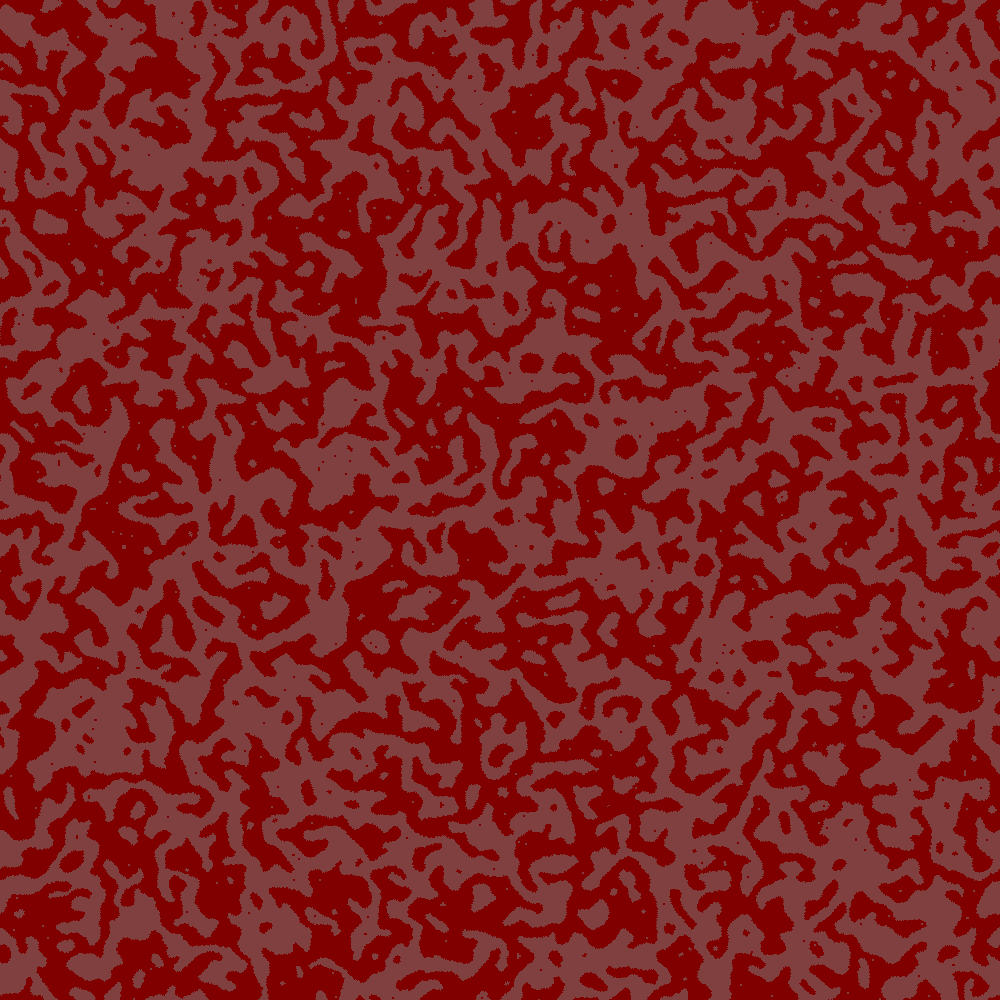
\includegraphics[width=0.5\textwidth]{./images/marco_teorico/automatas_celulares/Anneal.png}
        \caption{Evoluci\'on del aut\'omata celular \textit{Anneal}}
        \label{fig:anneal}
    \end{figure}
    \clearpage
    \subsubsection{Entrop\'ia de Shannon}
\label{sec:Entriopia}
    La entrop\'ia de Shannon es un concepto fundamental en la teor\'ia de la informaci\'on, 
        que se utiliza para medir la incertidumbre en una variable aleatoria. La entrop\'ia en si 
        es el grado de informaci\'n/desinformaci\'on que tenemos en un sistema. Es decir que cuanta m\'as
        informaci\'on tengamos de un sistema, menor ser\'a la entrop\'ia y viceversa. La entrop\'ia de Shannon, 
        nombrada as\'i por Claude Shannon\cite{Shannon1948}, se define mate la suma negativa de las probabilidades de cada
        posible valor de la variable aleatoria multiplicada por el logaritmo de la probabilidad de ese valor. Esta
        definici\'on es la siguiente:
        \begin{equation}
            H(X) = -\sum_{i=1}^{n} p(x_i) \log_b p(x_i)
        \end{equation}
    \vskip 0.5cm
    Donde $X$ es una variable aleatoria discreta, $p(x_i)$ es la probabilidad de que la variable aleatoria 
        $X$ tome el valor $x_i$ y $b$ es la base del logaritmo. En el caso de que la base del logaritmo sea 2, 
        la unidad de medida de la entrop\'ia ser\'an los bits. En el caso de que la base del logaritmo sea $e$,
        la unidad de medida de la entrop\'ia ser\'an los nat. Y en el caso de que la base del logaritmo sea 10, 
        la unidad de medida de la entrop\'ia ser\'an los dits.
    \vskip 0.5cm
    En nuestro caso en particular usamos bits como unidad de medida de la entrop\'ia, ya que lo usamos para saber que tipo de comportamiento
        tiene el aut\'omata celular. Es decir, si la entrop\'ia es alta, entonces el aut\'omata celular tiene un comportamiento ca\'otico, y si 
        la entrop\'ia es baja, entonces el aut\'omata celular tiene un comportamiento ordenado.
    \vskip 0.5cm
    Como vimos en ejemplo anterior, el aut\'omata celular \textit{Anneal} podemos observar r\'apidamente su entrop\'ia
        en la figura \ref{fig:annealEntropia}: 
        \begin{figure}[h]
            \centering
            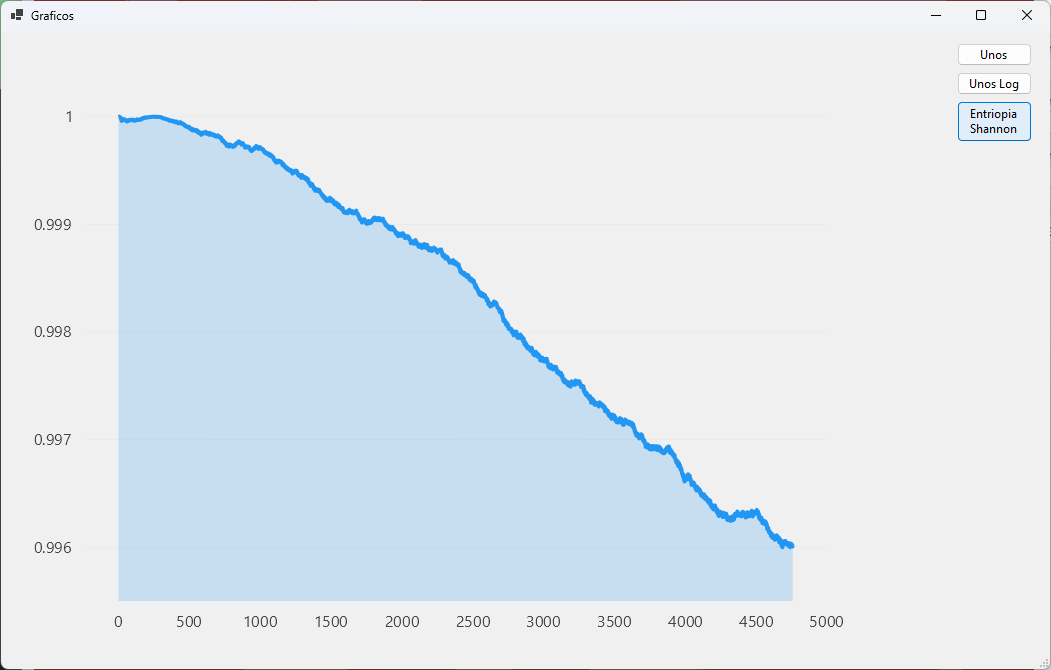
\includegraphics[width=0.5\textwidth]{./images/marco_teorico/automatas_celulares/Anneal5kShann.png}
            \caption{Entrop\'ia del aut\'omata celular \textit{Anneal} en 5000 generaciones}
            \label{fig:annealEntropia}  
        \end{figure}
    \subsubsection{Sistemas Din\'amicos}
\label{sec:SistemasDinamicos}
    La teor\'ia de Sistemas Din\'amicos puede considerarse una forma de describir c\'omo un determinado estado
        se transforma o evoluciona en otro a lo largo del tiempo, es decir, c\'omo evoluciona un sistema en el tiempo.
        La teor\'ia de Sistemas Din\'amicos se puede aplicar a cualquier \'area de la ciencia, como por ejemplo,
        la biolog\'ia, la econom\'ia, la f\'isica, la qu\'imica, etc. En nuestro caso en particular, la teor\'ia de
        Sistemas Din\'amicos se aplica a los aut\'omatas celulares, ya que los aut\'omatas celulares son sistemas
        din\'amicos discretos.
    \vskip 0.5cm
    Nos referimos a sistemas din\'amicos discretos cuando el tiempo es discreto. Con los aut\'omatas celulares
        podemos ver que el tiempo es discreto, ya que el tiempo se mide en generaciones. Es decir, en cada generaci\'on
        el aut\'omata celular evoluciona de un estado a otro. En la Figura \ref{fig:automataCelularEvolucion} podemos
        ver un ejemplo de la evoluci\'on de un aut\'omata celular en el tiempo:
        \begin{figure}[h]
            \centering
            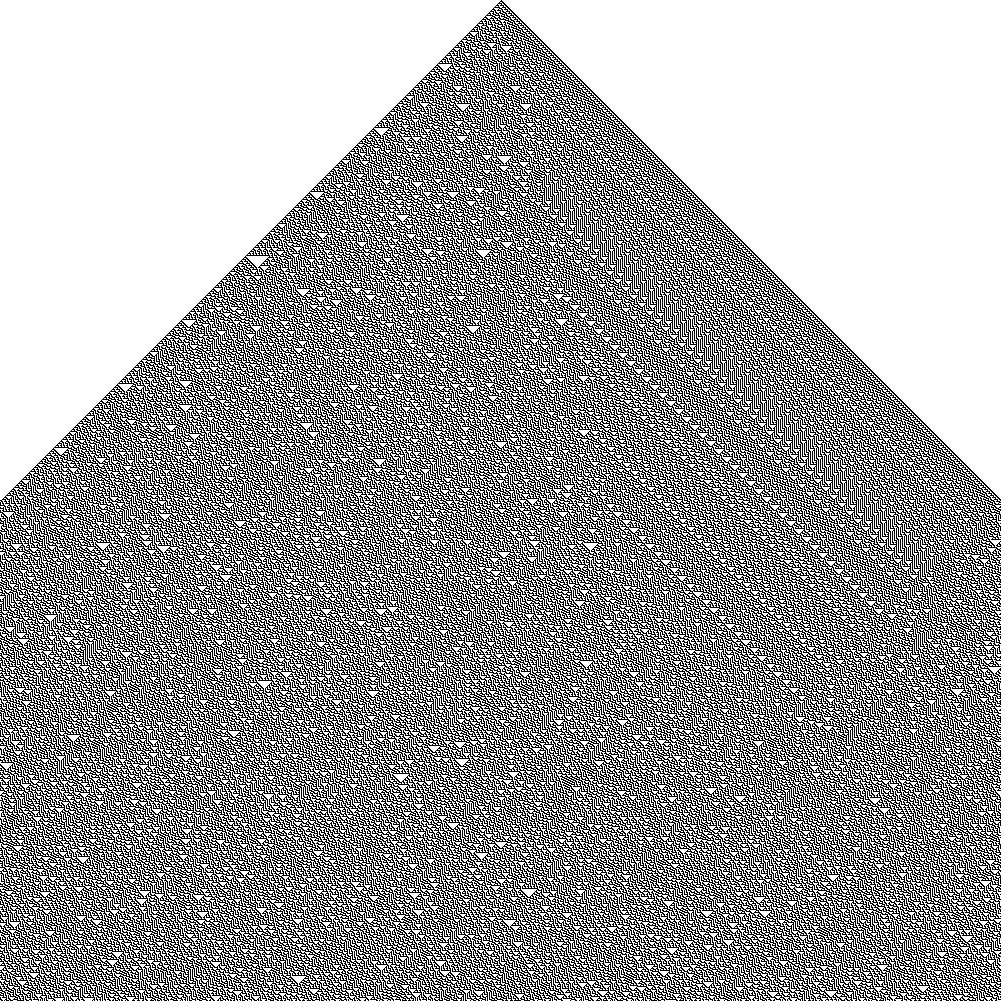
\includegraphics[width=0.5\textwidth]{./images/marco_teorico/automatas_celulares/Regla30-1000Gen.png}
            \caption{Evoluci\'on de la regla 30 en 1000 generaciones o pasos de tiempo}
            \label{fig:automataCelularEvolucion}
        \end{figure}
    \vskip 0.5cm
    No daremos una explicaci\'on m\'as en profundidad de los sistemas din\'amicos, ya que no es el objetivo de este
        trabajo. Para m\'as informaci\'on sobre sistemas din\'amicos y caos, se recomienda leer \cite{Ott1993} y tambi\'en \cite{Luenberger1979}.
        Sin embargo, lo que s\'i es importante mencionar es que los sistemas din\'amicos pueden ser clasificados,
        en este caso nos enfocaremos en los sistemas triviales, los sistemas complejos y los sistemas ca\'oticos.
    \vskip 0.5cm
    Esto lo hacemos con el prop\'osito de poder clasificar el comportamiento de nuestro aut\'omata celular (Physarum Polycephalum)
        en base a su comportamiento. Es decir, si el aut\'omata celular se comporta de manera trivial, compleja o ca\'otica.
        Para esto, primero daremos una breve explicaci\'on de cada uno de estos tipos de sistemas din\'amicos. A su vez, 
        quisi\'eramos destacar que para hacer nuestra clasificaci\'on o determinar el tipo de comportamiento tiene nuestro aut\'omata
        celular usaremos una gr\'afica en la cual podamos observar la Entrop\'ia de Shannon en funci\'on del tiempo. Ya que para
        poder usar como m\'etodo de clasificaci\'on los atractores, requerimos que la cantidad de estados en el Physarum Polycephalum
        es: $\mathbb{P} = \{x \in \mathbb{Z}| 0 \leq x \leq 8\}$ entonces es $S = \mathbb{P}$ y por lo tanto su funci\'on de transici\'on es: 
        $f: \mathbb{P} \rightarrow \mathbb{P}$ o sea $f: \mathbb{P}^{N} \rightarrow \mathbb{P}$ donde $N$ es la vecindad del aut\'omata celular.
        Por lo tanto, la funci\'on de transici\'on es una funci\'on de $\mathbb{P}^{9}$, 
        dandonos como resultado un total de $9^{9}$ o sea 387,420,489 estados posibles. Por lo tanto, no es posible graficar todos los
        estados posibles del aut\'omata celular.
    \vskip 0.5cm
    Ahora si, daremos una breve explicaci\'on de los sistemas mencionados anteriormente:
    \begin{itemize}
        \item \textbf{Sistemas Triviales:} Son sistemas que no tienen comportamiento complejo, es decir, son sistemas que
            tienen un comportamiento predecible. Por ejemplo, un p\'endulo simple, ya que su movimiento es peri\'odico y predecible.
        \item \textbf{Sistemas Complejos:} Son sistemas que tienen un comportamiento complejo, es decir, son sistemas que
            tienen un comportamiento impredecible debido a su sensibilidad a las condiciones iniciales y a la presencia de interacciones no 
            lineales.  Por ejemplo, el clima, ya que es imposible predecir el clima con exactitud.
        \item \textbf{Sistemas Ca\'oticos:} Los sistemas ca\'oticos son un subconjunto de sistemas complejos que son extremadamente sensibles 
            a las condiciones iniciales. Peque\~nas variaciones en las condiciones iniciales pueden llevar a resultados completamente diferentes en el
            tiempo. Los sistemas ca\'oticos pueden parecer aleatorios y desordenados, pero en realidad est\'an gobernados por ecuaciones matem\'aticas 
            deterministas. Un ejemplo cl\'asico de sistema ca\'otico es el sistema de doble p\'endulo, donde el movimiento se vuelve impredecible y 
            altamente sensible a las condiciones iniciales despu\'es de un corto per\'iodo de tiempo.
    \end{itemize}
